%%%%%%%%%%%%%%%%%%%%%%%%%%%%%%%%%%%%
% Using KTHEEtitlepage_ex.tex
%
% Example of how to use the KTHEEtitlepage package.
% 
% First Version : Mats Bengtsson,  7/8 2006
% Version 2 : Sunil Kallur Ramegowda, 8/3/2015
%%%%%%%%%%%%%%%%%%%%%%%%%%%%%%%%%%%%
\documentclass[12pt,a4paper]{article}

\usepackage[exjobb]{KTHEEtitlepage}
\usepackage{url}
\usepackage{tocloft}
\usepackage{hyperref}
\usepackage{filecontents,lipsum}
\usepackage{tocloft}
\renewcommand{\cftsecleader}{\cftdotfill{\cftdotsep}}
\usepackage[noadjust]{cite}
\graphicspath{{pictures/}}
\usepackage{booktabs}
\usepackage[table,xcdraw]{xcolor}

% Packages used in the main document for this particular example:
\usepackage{url}
\usepackage{tocloft}
\usepackage{hyperref}
\hypersetup{%
    pdfborder = {0 0 0}
}

\usepackage[exjobb]{KTHEEtitlepage}


\begin{document}
% Information to appear on the title page:
\ititle{Lumingo : Smart Backup Systems }
\isubtitle{}
\iauthor{- Sunil Kallur Ramegowda}

\idate{2015}


\iaddress{ICT Labs\\
  Major in Embedded Platforms\\
  Kungliga Tekniska H�gskolan}
%\irefnr{IR-EE-Dummy 2000:099}
\makeititle

% Everything below is exactly as for a normal document and 
% the layout of that document should not be affected in any
% way by the title page.

\title{Lumingo : Smart Backup Systems}
\author{Sunil Kallur Ramegowda}

\maketitle
\pagenumbering{roman}


\begin{abstract}
  The objective of this minor thesis is to perform the Literature study,Market research,competitor analysis, Hardware implementation and Result analysis of the Smart backup Systems.Electrical energy is the need for development. There are many ways of generating the electricity commercially like Hydroelectric power plants,Wind Mills,Nuclear Reactors,Solar Panels,Thermal reactors etc. Because of avoiding the hazardous effects from the Nuclear and Thermal power plants most of the nations are concentrating on renewable sources of energy like Solar and Windmills. This is also leading to the decentralization of the power generation into small grid like structure. The maintenance of these small grids centrally will give us more options of generating and utilizing the energy in a more efficient way.\\
  
  Grid based electricity manufacturing is already an existing technology in most of the developed countries in Europe like Germany,Estonia,\\Sweden etc. The Grids are locally managed using the SCADA PLC programming. The control decisions are all local and the real time decision based on the overall available data in the grids are not considered in the present techniques.\\
  
  Reaching the Grid owners or having access to the grid data is bit difficult without being in the industry. We as a team LuminGo have considered this as our proposal and have got the grant to show the first prototype to the SpeedUp Europe Accelerator program. The algorithm which will help to make the new IOT (Internet of Things) based technology in cleantech Energy is being supported by the European Union.   
\end{abstract}

\addcontentsline{toc}{section}{Abstract}
\cleardoublepage




%\phantomsection

\renewcommand\contentsname{\centerline{\underline{\underline{Table of Contents}}}}
\tableofcontents
\addcontentsline{toc}{section}{Table of Contents}
\cleardoublepage


%\renewcommand\listfigurename{List of Figures}

\listoffigures
\addcontentsline{toc}{section}{List of Figures}
\cleardoublepage

\renewcommand\listtablename{List of Tables}
\listoftables
\addcontentsline{toc}{section}{List of Tables}
\clearpage



\pagenumbering{arabic}

\section{Introduction}

Electrical Energy is a vital need for everyday life as we are depending on machines where most of them need electrical energy to perform their task.There are many ways of generating electricity and then storing it to use it according to the need. Batteries are used to store Electrical energy in the form of chemical energy, but the innovations in battery technologies are still not advanced and is a big problem for the society.So efficient use of the generated power and its storage are necessary.Renewable sources of energy like Solar panel and Bio Mass are famous as they do not have extracts which are harmful to the nature when compared to the Nuclear power plants.Generating power using technologies like Wind,Solar,Bio Mass etc are feasible and countries like India,Uganda,Germany etc are supporting for such implementations.\\

When the grids increase in numbers their maintenance and operational decisions need to be smart for optimized and efficient power generation and utilization.In the present day there are challenges because of unreliable grids and power generators which generate frequent power outages when the power production does not meet the requirement. Our concept is a smart grid system that will integrate the 
individual backup power systems in the overall grid management.\\

There are many algorithms designed for making the overall system efficient and robust. We need to collect data from each of the Backup systems and our algorithm will make dynamic decisions in the central server.We are proposing to make the complete system Smart using the FIWARE cloud platform which is being sponsored from the European Union. I am working as one among the CTO who has to research and design the Embedded Hardware to capture the data and also to send it to the cloud using GPRS/GSM technology for further processing.



\clearpage


\section{Literature and competitor Analysis}
M2M(Machine to Machine) interaction is expected to be the next generation of research goal in all sectors to make the human life better.Semiconductors,  Networking and Software firms are building the next products which support for the easy integration of such applications.The cost of adding connectivity to a device has fallen significantly (less than 5dollars!).The energy consumption of these tiny modules which communicate with radio is also significantly reduced such that they are able to work standalone with batteries for almost a year\cite{maulik}.Sensors which collects such data and store them in real time or near real time are of great importance for development of new applications with different market strategies. The energy sector is also facing such fast integration of technological advancements for the better management of electrical energy.The need for integrating all such devices to be able to control,monitor and switch from remote location based on their status leads to infinite possibilities of innovation.\\

\begin{figure}[!htb]
    \centering
    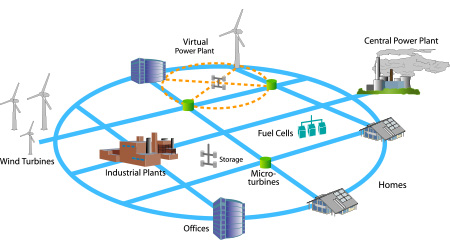
\includegraphics[scale=1]{smartgrid2}
    \caption{Smart Grid concept\cite{smartgrid}}
    \label{fig:Fig1}
\end{figure}


The Energy generation and distribution model is different in each country. But the need for making optimal usage of the produced energy exist everywhere.Making the Grids  "Smart" is now the need of the society.The smart metering is one part of the Smart grid concept wherein the meters at individual location will collect and store the data in central cloud for further processing or usage for different applications in future.The installation and replacements of smart meters alone in Europe has the range of 12 to 17 million units\cite{BergInsight}.The estimated growth rate of smart meters is 18.5 percent between 2013 and 2019 to reach 170.1 million units at the end of the period.According to the statistics\cite{BergInsight}, thirteen European countries had developed regulatory road maps for the full scale introduction of the smart electricity meters.\\ 



As in Fig.~\ref{fig:Fig1},A smart Grid can be defined as the process of efficient use of energy from the point of generation to distribution till consumption at the consumer end.Therefore intelligence needs to be build to make decisions on real time or near real time for the system to work.This needs the sensors and actuator systems to collect data and take action respectively.All forms of energy generation and consuming units can be integrated into this system for the best efficient algorithms to make intelligent decisions.\\




\begin{figure}[!htb]
    \centering
    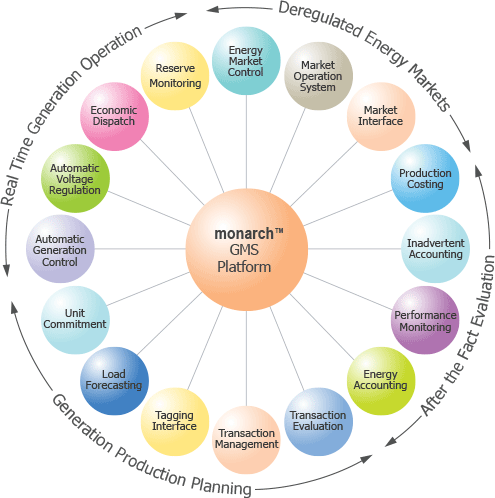
\includegraphics[scale=0.5]{GMS-platform}
    \caption{Grid Software Functions\cite{smartgrid}}
    \label{fig:Fig2}
\end{figure}




The Smart grid software which is presently used are the SCADA based systems. One such system from the company OSII is shown in Fig.~\ref{fig:Fig2}.There are many functionalities and decisions which can be performed based on the data collected or from the connected systems.The general decision like where the power outage has to happen based on location or number of energy consumptions can be achieved by the grid owners in an autonomous way or even manual way.

The Fig.~\ref{fig:Fig3} explains the statistics of the Smart grid progress in Europe performed by Joint Research Centre,Institute for Energy and Transport(\url{http://ses.jrc.ec.europa.eu/smart-grids-observatory}).As indicated the overall market in last one decade is amounting to 3.15 billion Euros of investment.\\

\begin{figure}[!htb]
    \centering
    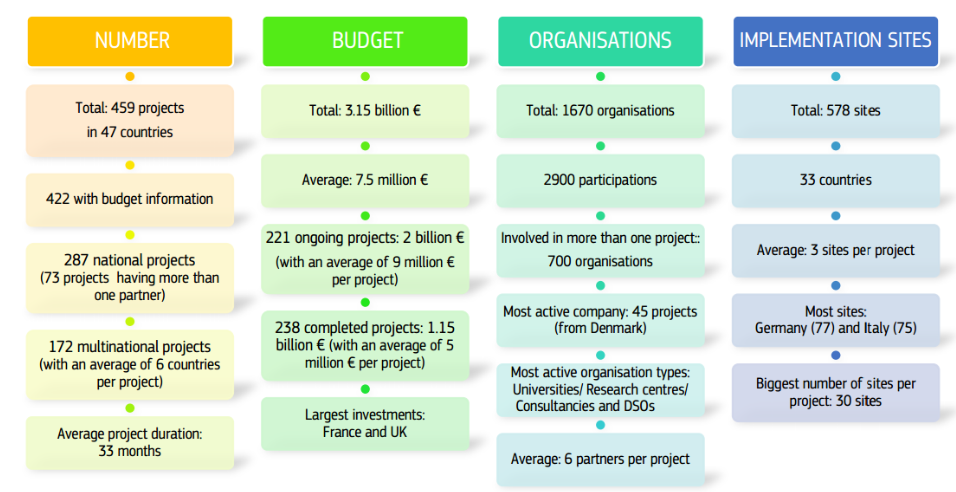
\includegraphics[scale=0.45]{EU_report}
    \caption{Survey of EU Smart Grid in 2014 \cite{EUreport}}
    \label{fig:Fig3}
\end{figure}

% Please add the following required packages to your document preamble:
% \usepackage{booktabs}
% \usepackage[table,xcdraw]{xcolor}
% If you use beamer only pass "xcolor=table" option, i.e. \documentclass[xcolor=table]{beamer}


There are many big companies like ABB\cite{ABB},Schneider\cite{Schneider} in this market which hold the major equipments sales. The new startup define their business model such that they become collaborative partners than competitors,which is the similar case with LuminGo AB.We are concentrating to enter the market through developing countries like India,Pakistan and African countries.Based on the funding we have received from the European Union, part of it is being spent on the hardware prototype development.The hardware is similar to the smart meter which also includes the actuators to perform connect/disconnect operation from remote location i.e through the grid management software.The business model also concentrates on controlling the gas and water meters from the central location as the overall system is similar except the actuation hardware at the consumer end.\\

The state of the art in the developing countries is similar to the path of technological advancement in developed countries.Pamoja AB which is the parent company of LuminGo AB has 2 grids setup in Uganda which are used for rural electrification\cite{pamoja}.The idea of optimally utilizing the electricity generated necessitated the  need of a central control.Research on the need and present day problem faced by the electricity grids in Uganda shows an average estimate of 16k power outages in Uganda. With the Grid Management software with the necessary hardware for controlling it can make the system more reliable and efficient.We are planning to show the proof of concept to give the projection of the savings to the energy companies.\\

Recent developments in India has also shown the adaption of these techniques to manage the system more efficiently.Cyan Technology, an UK based company has got the first public pilot project in the Southern Indian region.This involves the intstallation of 21k smart meters replacing the old technology meters.These smart meters can perform more functions and it becomes easier to monitor the system.The Overall estimate of the project is greater than 1M Pounds\cite{Cyan}.The Smart cities project initiated by the Government of India\cite{india}, has also proposed the integration of energy management concept which results in the investment. 

\clearpage


\section{Product and Market Entry}








\begin{filecontents*}{references.bib}
    
    
    @misc{maulik,
        author = {Maulik,Sunil},
        title = {Trends in infrastructure: the Internet of Things},
        howpublished = {\url{http://www.oracle.com/us/corporate/profit/big-ideas/012314-smaulik-2112685.html}},
        year = {2014},
        note = {Accessed: 2015-04-20}
    }
    
    @misc{BergInsight,
        author = {Ryberg Tobias},
        title = {Smart Metering in Europe },
        howpublished = {\url{http://www.berginsight.com/ReportPDF/ProductSheet/bi-sm10-ps.pdf}},
        year = {2014},
        note = {Accessed: 2015-04-20}
    }
     @misc{smartgrid,
         author = {},
         organization = {OSI,powering the future},
         title = {Smart grid concept },
         howpublished = {\url{http://www.osii.com/solutions/initiatives/smartgrid.asp}},
         year = {2014},
         note = {Accessed: 2015-04-20}
        }
     @misc{EUreport,
         author = {},
         organization = {Joint Research Centre,Institute for Energy and Transport},
         title = {Smart Grid Projects Outlook 2014 },
         howpublished = {\url{http://ses.jrc.ec.europa.eu/smart-grids-observatory}},
         year = {2014},
         note = {Accessed: 2015-04-20}
        }
        
        @misc{EUreport,
            author = {},
            title = {ABB Ltd },
            howpublished = {\url{ http://new.abb.com/about/technology/data-centers/gridconnection}},
            year = {2015},
            note = {Accessed: 2015-04-21}
        }
        @misc{ABB,
            author = {},
            title = {ABB Ltd },
            howpublished = {\url{ http://new.abb.com/about/technology/data-centers/gridconnection}},
            year = {2015},
            note = {Accessed: 2015-04-21}
        }
         @misc{Schneider,
             author = {},
             title = {Schneider Electric},
             howpublished = {\url{ http://www2.schneider-electric.com/sites/corporate/en/products-services/smart-grid-solutions/smart-grid-solutions.page}},
             year = {2015},
             note = {Accessed: 2015-04-21}
            }
    @misc{pamoja,
        author = {},
        title = {Pamoja AB},
        howpublished = {\url{ http://pamoja.se/}},
        year = {2011},
        note = {Accessed: 2015-04-21}
    }
    
    @misc{cyan,
        author = {},
        title = {Cyan Technology},
        howpublished = {\url{http://www.cyantechnology.com/articles/1m-order-public-utility-smart-metering-project-india/}},
        year = {2011},
        note = {Accessed: 2015-04-21}
    }
    
    @misc{india,
        author = {},
        title = {India: Smart Cities},
        howpublished = {\url{http://indiansmartcities.in/Site/index.aspx}},
        year = {2011},
        note = {Accessed: 2015-04-21}
    }
    
    
   
    
    
\end{filecontents*}
\bibliographystyle{ieeetr}
\bibliography{references}
\addcontentsline{toc}{section}{References}


\end{document}
